\chapter{Methodology}
\label{cha:methodology}
This chapter presents two parallel BFS implementations. \cref{sec:mergedcsr} describes a cache-optimized implementation using the MergedCSR data structure. The code is implemented in C++ using the OpenMP parallelization framework. \cref{sec:pthreads} describes an explicitly parallelized BFS implementation in C using the pthreads parallel execution model.

\section{Cache-optimized BFS using the MergedCSR data structure}
\label{sec:mergedcsr}
The performance of a Top-Down BFS traversal on a standard Compressed Sparse Row (CSR) representation is often constrained by memory latency. For each vertex explored, the algorithm must perform scattered memory accesses to three distinct data structures: the \rowptr{} array to find the offset of the adjacency list, the \colidx{} array to retrieve the neighbors, and a separate distances array to check the visited status and store the new distance. These disjoint accesses frequently lead to cache misses, as the data required to process a single vertex is not co-located in memory.

\subsection{Design and Memory Layout of MergedCSR}

To mitigate scattered memory accesses, the MergedCSR format merges the \rowptr{} and \colidx{} arrays into a single contiguous structure. The format proposed in this work extends this data structure by integrating algorithm-specific metadata directly into the graph's memory layout. In this new format, the adjacency list for each vertex is prepended with two metadata fields: the vertex's degree and its distance from the source vertex. The entire graph is thus stored in a single, large array where each vertex's data block is structured as: \texttt{[degree, distance, neighbor\_1\_idx, neighbor\_2\_idx, ...]}. Since each vertex's data block in MergedCSR is expanded by two elements (for degree and distance), the offsets for each subsequent vertex will be larger. A new \rowptr{} array is therefore necessary to correctly index into the start of each vertex's block within the new, larger structure. The space complexity for the MergedCSR array is thus \bigO{2|V| + |E|} elements. An example of the MergedCSR structure is shown in \cref{fig:improved_merged}, the pseudocode for converting from a standard CSR representation to MergedCSR is outlined in \cref{alg:convert_to_merged_csr}, and the pseudocode to extract the distances from the MergedCSR is outlined in \cref{alg:extract_distances}.

\begin{figure}
    \centering
    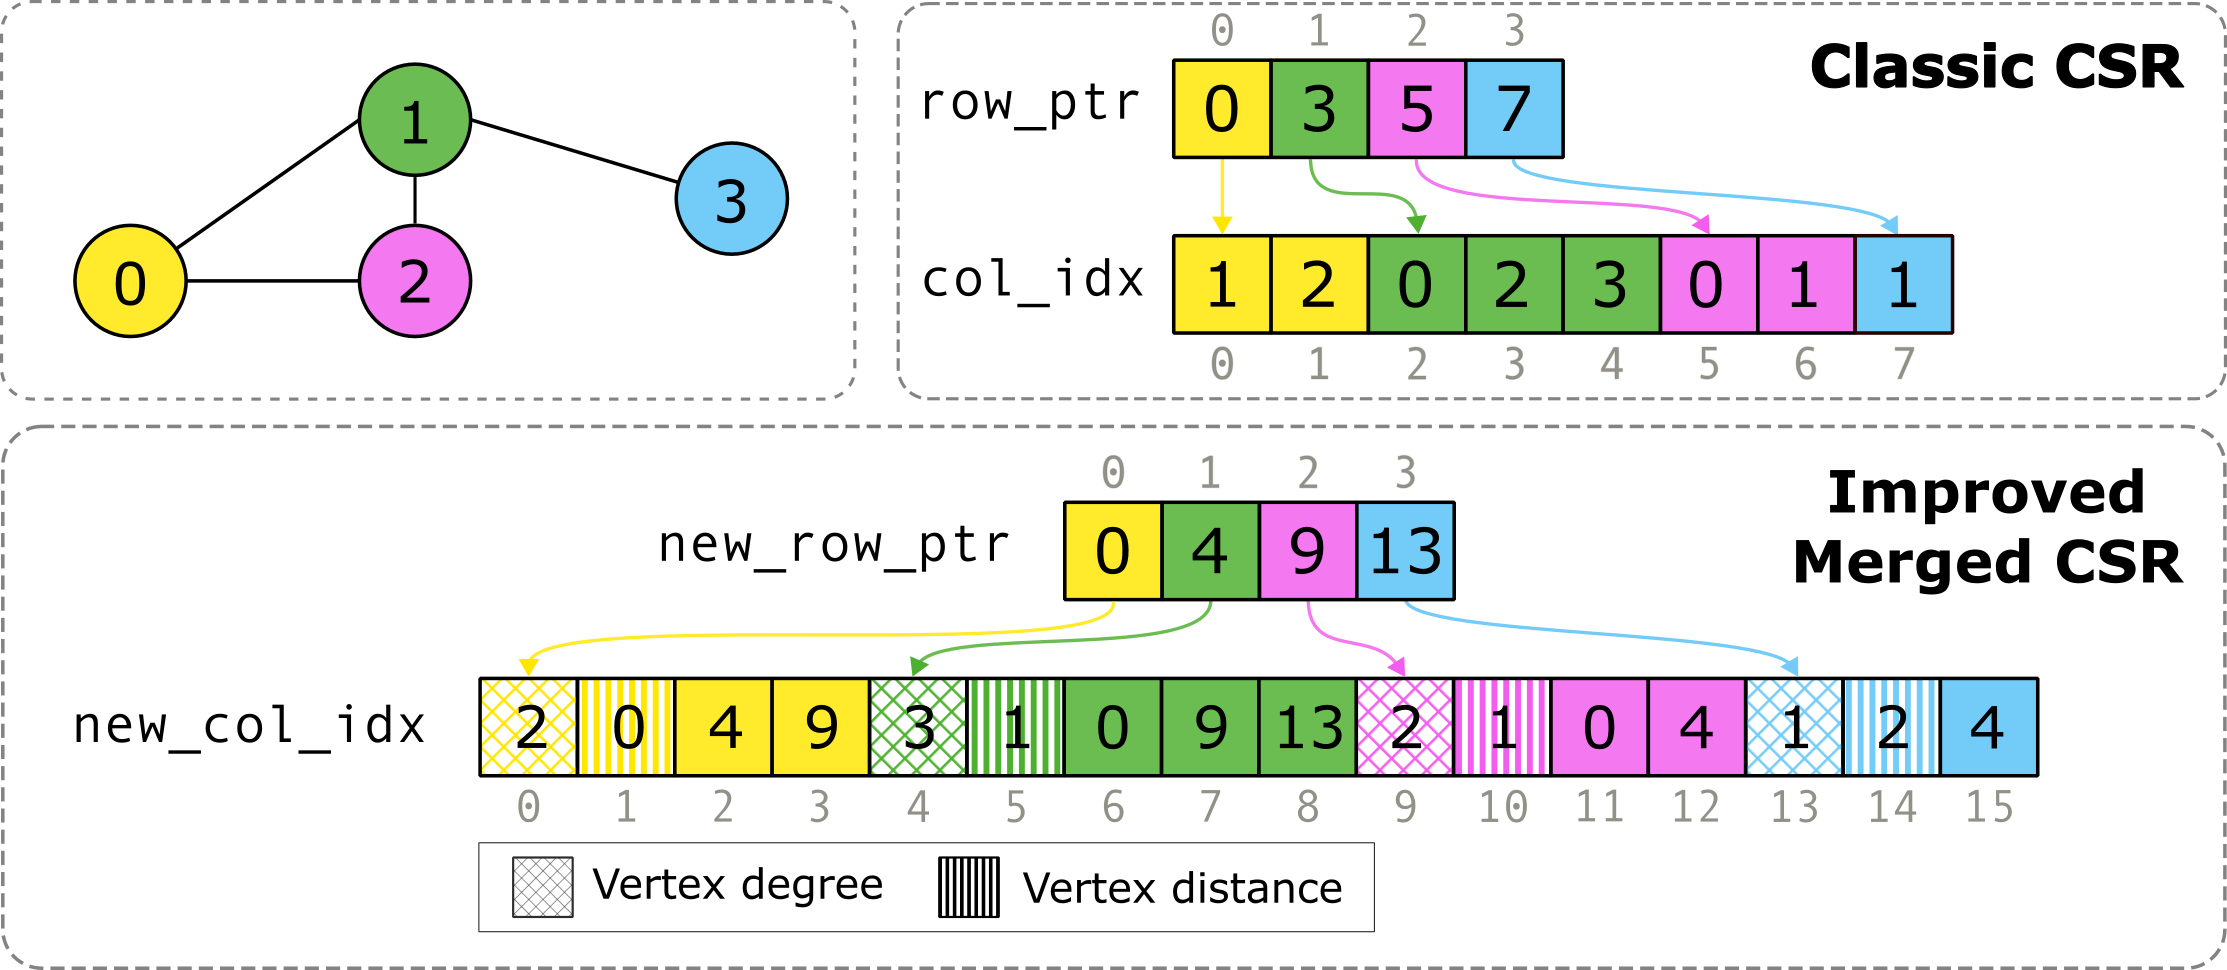
\includegraphics[width=0.8\linewidth]{images/csr_improved.png}
    \caption{An example of the improved MergedCSR structure.}
    \label{fig:improved_merged}
\end{figure}

\begin{algorithm}[H]
    % --- Define Inputs and Outputs ---
    \KwIn{
        $row\_ptr$: An array of row pointers for a standard CSR graph.\\
        $col\_idx$: An array of column indices for a standard CSR graph.\\
        $num\_vertices$: The total number of vertices in the graph.
    }
    \KwOut{
        $new\_row\_ptr$: The new row pointer array for the MergedCSR structure.\\
        $merged\_csr$: The new data structure containing degrees, distances, and neighbors.
    }
    
    \caption{Conversion to a Merged CSR Representation}
    \label{alg:convert_to_merged_csr}

    % Initialization
    $merged\_csr \gets \text{new int} [2 \times num\_vertices + |col\_idx|]$\;
    $new\_row\_ptr \gets \text{new int} [num\_vertices + 1]$\;
    $cursor \gets 0$\;

    \BlankLine % Adds a little visual space
    
    % Main loop over all vertices
    \For{$i \gets 0$ \KwTo $num\_vertices - 1$}{
        $new\_row\_ptr[i] \gets cursor$
        \tcp*{Update position of vertex $i$ in the new structure}
        \BlankLine
        $degree \gets row\_ptr[i+1] - row\_ptr[i]$\;
        $merged\_csr[cursor] \gets degree$ \tcp*{Initialize degree}
        $merged\_csr[cursor + 1] \gets \infty$ \tcp*{Initialize distance}
        $cursor \gets cursor + 2$ \tcp*{Offset cursor by number of metadata cells}

        \tcp{Copy neighbors of vertex $i$}
        \For{$j \gets row\_ptr[i]$ \KwTo $row\_ptr[i+1] - 1$}{
            \tcc{Retrieve the ID of this neighbor from the original col\_idx array}
            $neighbor\_id = col\_idx[j]$\;
            \tcc{Calculate the starting index of this neighbor's data block. Account for its original offset (row\_ptr[neighbor\_id]) plus the two metadata slots added for every vertex that comes before it (2 * neighbor\_id)}
            $new\_position \gets row\_ptr[neighbor\_id] + 2 * neighbor\_id$\; 
            \tcc{Store the calculated pointer in the new structure}
            $merged\_csr[cursor] \gets new\_position$\;
            $cursor \gets cursor + 1$ \tcp*{Advance the cursor to the next available position}
        }
    }
    $new\_row\_ptr[num\_vertices] \gets cursor$\;
    
    \BlankLine
    \KwRet{$new\_row\_ptr, merged\_csr$}\;
\end{algorithm}
\begin{algorithm}[H]
    \KwIn{
        $merged\_row\_ptr$: The row pointer array for the MergedCSR structure. \\
        $merged\_csr$: The MergedCSR data array containing metadata and neighbors. \\
        $num\_vertices$: The total number of vertices.
    }
    \KwOut{
        $distances$: An array populated with the distance of each vertex from the source.
    }
    
    \caption{Distance Extraction from MergedCSR}
    \label{alg:extract_distances}

    \BlankLine
    \For{$i \gets 0$ \KwTo $num\_vertices - 1$}{
        $offset \gets merged\_row\_ptr[i]$ \tcp*{Get start index for vertex $i$'s data block}
        $distances[i] \gets merged\_csr[offset + 1]$ \tcp*{Copy final distance from metadata}
        $merged\_csr[offset + 1] \gets \infty$ \tcp*{Reset distance in MergedCSR for next run}
    }
    \BlankLine
    
    \KwRet{$distances$}\;
\end{algorithm}

This layout is explicitly designed to exploit spatial locality. When the BFS algorithm accesses a vertex to check or update its distance, the CPU hardware will load the corresponding cache line. Because the vertex's degree and its first few neighbors are now stored immediately after the distance field, it is highly probable that this single memory fetch will also load the beginning of the vertex's adjacency list into the cache. This effectively prefetches the data required for the next frontier expansion, thereby reducing or eliminating subsequent cache misses that would have been necessary with the standard CSR format.

\subsection{Traversal Algorithm and Implementation Details}

The BFS algorithm implemented using the MergedCSR data structure is level-synchronous. This means that all vertices at a given distance $d$ from the source are fully explored before the algorithm proceeds to discover vertices at distance $d+1$.

Due to the structure of the MergedCSR, this design is optimized exclusively for the Top-Down traversal step and precludes an efficient Bottom-Up implementation. The core operation of the Bottom-Up approach involves iterating over all unvisited vertices and checking if any of their neighbors reside in the current frontier. This check is performed efficiently using a bitmap of the frontier, which requires a direct mapping from a vertex ID to its corresponding bit in the bitmap. The MergedCSR format changes the indices in the adjacency lists and breaks the index-to-vertex-ID mapping. While one could search for each neighbor's original ID to query the bitmap, the computational overhead of this \bigO{|V|} lookup would negate any performance benefits of the Bottom-Up strategy. Therefore, to maximize the benefit of the improved data locality, only the Top-Down exploration strategy is employed.

Parallelism is introduced at each level of the traversal by partitioning the vertices of the current frontier among a team of OpenMP threads. The implementation follows the ``Thread-Local Frontiers'' with a ``Final Merge Step'' parallelization strategy (see \cref{sec:strategies} and \cref{fig:paral_merged}). This strategy is realized efficiently through a custom OpenMP reduction. Instead of having all threads contend for locks or use atomic operations to write to a single shared next-frontier, each thread populates its own private, thread-local version of the next frontier. At the end of the parallel exploration for that level, OpenMP automatically performs a final merge step to combine all the thread-local frontiers into a single, unified frontier for the next iteration.
\begin{minted}{cpp}
#pragma omp declare reduction(vec_add \
    : frontier : omp_out.insert(omp_out.end(), omp_in.begin(), omp_in.end()))
\end{minted}
This custom reduction instructs OpenMP on how to combine the thread-local frontiers at the end of the parallel loop: the contents of each thread's private frontier (\texttt{omp\_in}) are appended to the master frontier (\texttt{omp\_out}). This direct vector concatenation avoids the need for manual synchronization. The custom reduction is then applied to the for loop that iterates over the vertices in the frontier, as shown the the following listing.
\begin{minted}[xleftmargin=20pt, breaklines, linenos]{cpp}
#pragma omp parallel for reduction(vec_add : next_frontier) schedule(static) if (this_frontier.size() > 50)
for (const auto &v : this_frontier) {
  eidType end = v + 2 + DEGREE(v);
  // Iterate over neighbors
  for (eidType i = v + 2; i < end; i++) {
      eidType neighbor = merged_csr[i];
      // If neighbor is not visited, add to frontier
      if (DISTANCE(neighbor) == std::numeric_limits<weight_type>::max()) {
        if (DEGREE(neighbor) != 1) {
          next_frontier.push_back(neighbor);
        }
        // Set the neighbor's distance
        DISTANCE(neighbor) = distance;
      }
  }
}
\end{minted}

The outer loop is parallelized using the \texttt{schedule(static)} clause, which pre-allocates fixed-size chunks of the frontier to each thread. While graph traversal workloads are inherently irregular and can lead to load imbalance, empirical evaluation demonstrated that the low overhead of static scheduling consistently outperformed the more complex dynamic scheduling strategies offered by OpenMP.

Furthermore, parallelization is enabled only when the frontier size exceeds a threshold of 50 vertices. This optimization prevents the runtime overhead associated with creating and managing the thread team from outweighing the computational speedup on small workloads, for which sequential execution is faster.

\subsection{Postprocessing and Generality}

Once the BFS traversal is complete, the distance values are embedded within the MergedCSR structure. A final postprocessing step is required to extract these values into a standard distances array. This is accomplished with a simple parallel loop that iterates from $0$ to $|V|-1$, using the updated \rowptr{} to locate the distance field for each vertex and copy its value. The pseudocode of this procedure is outlined in \cref{alg:extract_distances}.

The same framework can be adapted to produce a parent array instead of a distance array. In this variation, the distance field in the MergedCSR structure is repurposed to store the parent ID of each vertex. The logic of the traversal remains largely the same, with the algorithm storing the ID of the discovering vertex instead of the new distance level.

\newpage

\section{Case study: Explicit parallelization of BFS using pthreads}
\label{sec:pthreads}

This section presents an alternative BFS implementation that avoids high-level parallelization frameworks and instead uses explicit thread management with the POSIX Threads (pthreads) library in C. This approach provides fine-grained control over thread lifecycle, work distribution, and synchronization. The design is built upon three core components: a persistent thread pool to minimize thread creation overhead, a chunk-based frontier with a work-stealing mechanism to dynamically balance the load, and a low-overhead, centralized barrier to ensure level-synchronous traversal. For its underlying graph representation, this implementation utilizes the cache-optimized Merged CSR data structure.

\subsection{The Chunk-Based Frontier}

The parallel frontier is managed by a set of data structures designed to minimize lock contention, reduce dynamic memory allocation overhead, and facilitate a dynamic work-stealing load balancing strategy. The design is composed of three primary structures: the \texttt{Chunk}, the \texttt{ThreadChunks} queue, and the top-level \texttt{Frontier} container. A schematic representation of the combined structures is shown in \cref{fig:frontier}.

\paragraph{The \texttt{Chunk} structure} This structure represents the atomic unit of work distributed among threads. The structure consists of a fixed-size block containing an array of vertex identifiers. The \texttt{CHUNK\_SIZE} constant defines the capacity of each block. This design choice amortizes the overhead associated with managing the frontier; instead of threads manipulating individual vertices in a shared queue, they acquire and process entire blocks of work at a time. The \texttt{next\_free\_index} field serves as a stack pointer, allowing the \texttt{Chunk} object to function as a Last-In, First-Out (LIFO) buffer. Vertices are pushed by placing them at this index and incrementing it, and popped by decrementing the index. When \texttt{next\_free\_index} is zero, the chunk is empty. This LIFO access pattern is cache efficient, as vertices that were just written to the chunk are also the first ones to be read and processed.

\begin{minted}{c}
typedef struct {
  ver_t vertices[CHUNK_SIZE];
  int next_free_index;
} Chunk;
\end{minted}

\paragraph{The \texttt{ThreadChunks} structure} This structure manages a dynamic array of pointers to a set of \texttt{Chunk} structures. The \texttt{top\_chunk} index makes the array function as a stack, while the \texttt{chunks\_size} field tracks the total allocated capacity of this array. If a thread's queue runs out of space (i.e., \texttt{top\_chunk} reaches \texttt{chunks\_size}), the chunks array is reallocated to double its previous capacity. This expansion strategy, which is implemented using the \texttt{realloc()} function, ensures that the cost of adding new chunks has amortized cost \bigO{1}. Similarly to the \texttt{Chunk} structure, this structure also acts as a LIFO stack to exploit temporal cache locality. During the frontier expansion phase of a BFS level, a thread creates and populates new chunks with newly discovered vertices. In the subsequent BFS level, the thread will pop the chunks to process them. Because the top chunks were the last to be inserted, they also have a higher probability of still residing in the thread's private L1 or L2 caches, therefore optimizing the cache usage. Each \texttt{ThreadChunks} structure contains also its own \texttt{pthread\_mutex\_t} lock. A thread must acquire this lock to add or remove a \texttt{Chunk} from its own queue. This same lock must be acquired also by any other thread attempting to "steal" a Chunk from this queue.

\begin{minted}{c}
typedef struct {
  Chunk **chunks;
  int chunks_size;
  int top_chunk;
  pthread_mutex_t lock;
} ThreadChunks;
\end{minted}

\paragraph{The \texttt{Frontier} structure} This structure consists of an array of pointers to \texttt{ThreadChunks} objects, providing a centralized point of access to each thread's individual work queue. This allows a work-stealing thread to iterate through all other threads and attempt to acquire work from their respective queues. The \texttt{Frontier} structure contains also a \texttt{thread\_chunk\_counts} array, which stores the number of active chunks per thread. This array provides a fast, lock-free snapshot of the entire system's work distribution. An idle thread can scan this array to quickly identify the busy threads and steal work from them, without incurring the high contention cost of acquiring each thread's mutex simply to inspect its queue size.

\begin{minted}{c}
typedef struct {
  ThreadChunks **thread_chunks;
  int *thread_chunk_counts;
} Frontier;
\end{minted}

\begin{figure}[h]
    \centering
    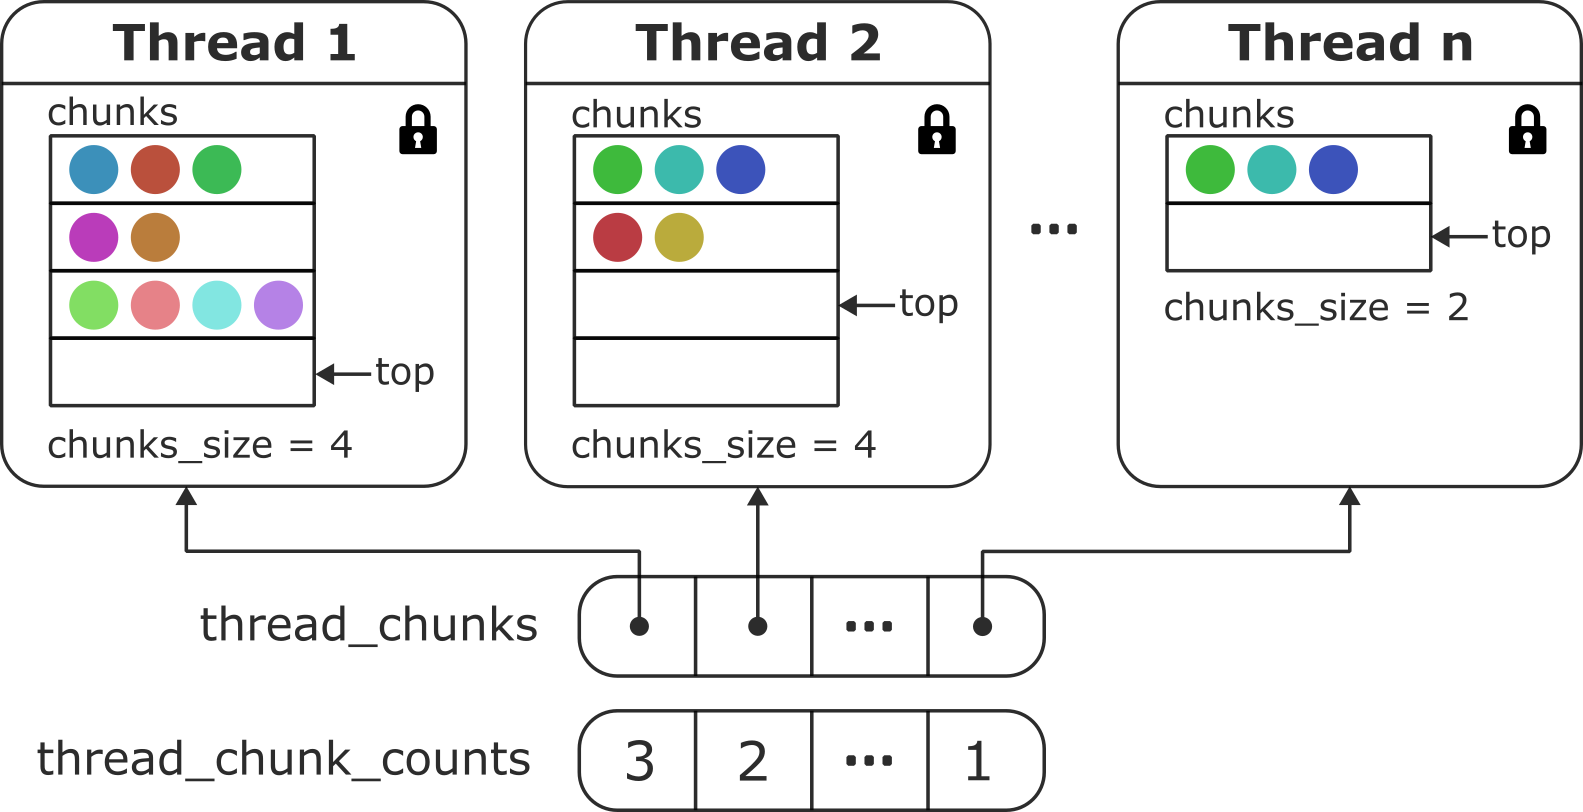
\includegraphics[width=0.7\linewidth]{images/frontier.png}
    \caption{An overview of the \texttt{Frontier} data structure for parallel BFS. The top-level \texttt{Frontier} structure contains pointers to each thread's private \texttt{ThreadChunks} work queue. Each \texttt{ThreadChunks} contains a stack of \texttt{Chunks}, with the top pointer indicating the next available slot in the stack. The colored circles represent the vertices contained in each chunk. Access to the \texttt{chunks} array is serialized by a dedicated mutex (represented by the lock icon). The auxiliary \texttt{thread\_chunk\_counts} array provides lock-free access to the number of chunks of each thread.}
    \label{fig:frontier}
\end{figure}

\subsection{Dynamic Load Balancing via Work-Stealing}

To counteract the inherent workload imbalance characteristic of irregular graph traversal, a dynamic work-stealing mechanism is implemented. This protocol allows idle threads to acquire work from busy threads.

A thread transitions from a "worker" to a "thief" state as soon as it has processed all the chunks in its own \texttt{ThreadChunks} queue. Once its own work queue is empty, it initiates the work-stealing protocol. First, the stealing thread iterates through the \texttt{thread\_chunk\_counts} array, looking for any thread whose chunk count is greater than one. This heuristic prevents excessive lock contention, particularly during phases of the BFS where the frontier is small. If the entire frontier consists of only a single chunk, this rule prevents all but one thread from repeatedly attempting to lock the same mutex, a phenomenon which would serialize execution and negate the benefits of parallelism.

Upon identifying a potential victim that satisfies this condition, the thief proceeds to attempt a steal. It first tries to acquire the victim thread's \texttt{pthread\_mutex\_t} lock. Once the lock is successfully acquired, the thief performs a second check on the victim's chunk count. This check is necessary to prevent a race condition; it is possible that another thief stole a chunk in the time between the initial lock-free check and the successful acquisition of the lock. If the victim thread still has more than one chunk available, the steal is executed. The thief decrements the victim's \texttt{top\_chunk} index to claim a chunk, and the corresponding value in the shared \texttt{thread\_chunk\_counts} array to ensure the global view of work distribution remains consistent. After these modifications, the thief releases the victim's lock and begins processing the vertices within the stolen chunk.

Upon finishing the stolen chunk, the thief thread re-initiates the work-stealing protocol, starting a new scan of the \texttt{thread\_chunk\_counts} array to find another victim. This loop continues until the thread performs a full scan of the \texttt{thread\_chunk\_counts} array and finds that all entries are zero. This state signifies that the entire frontier for the current level has been processed. At this point, the thread stop its execution for the current level and proceed to the synchronization barrier. The flowchart of the work-stealing protocol is shown in \cref{fig:workstealing}.

\begin{figure}[h]
    \centering
    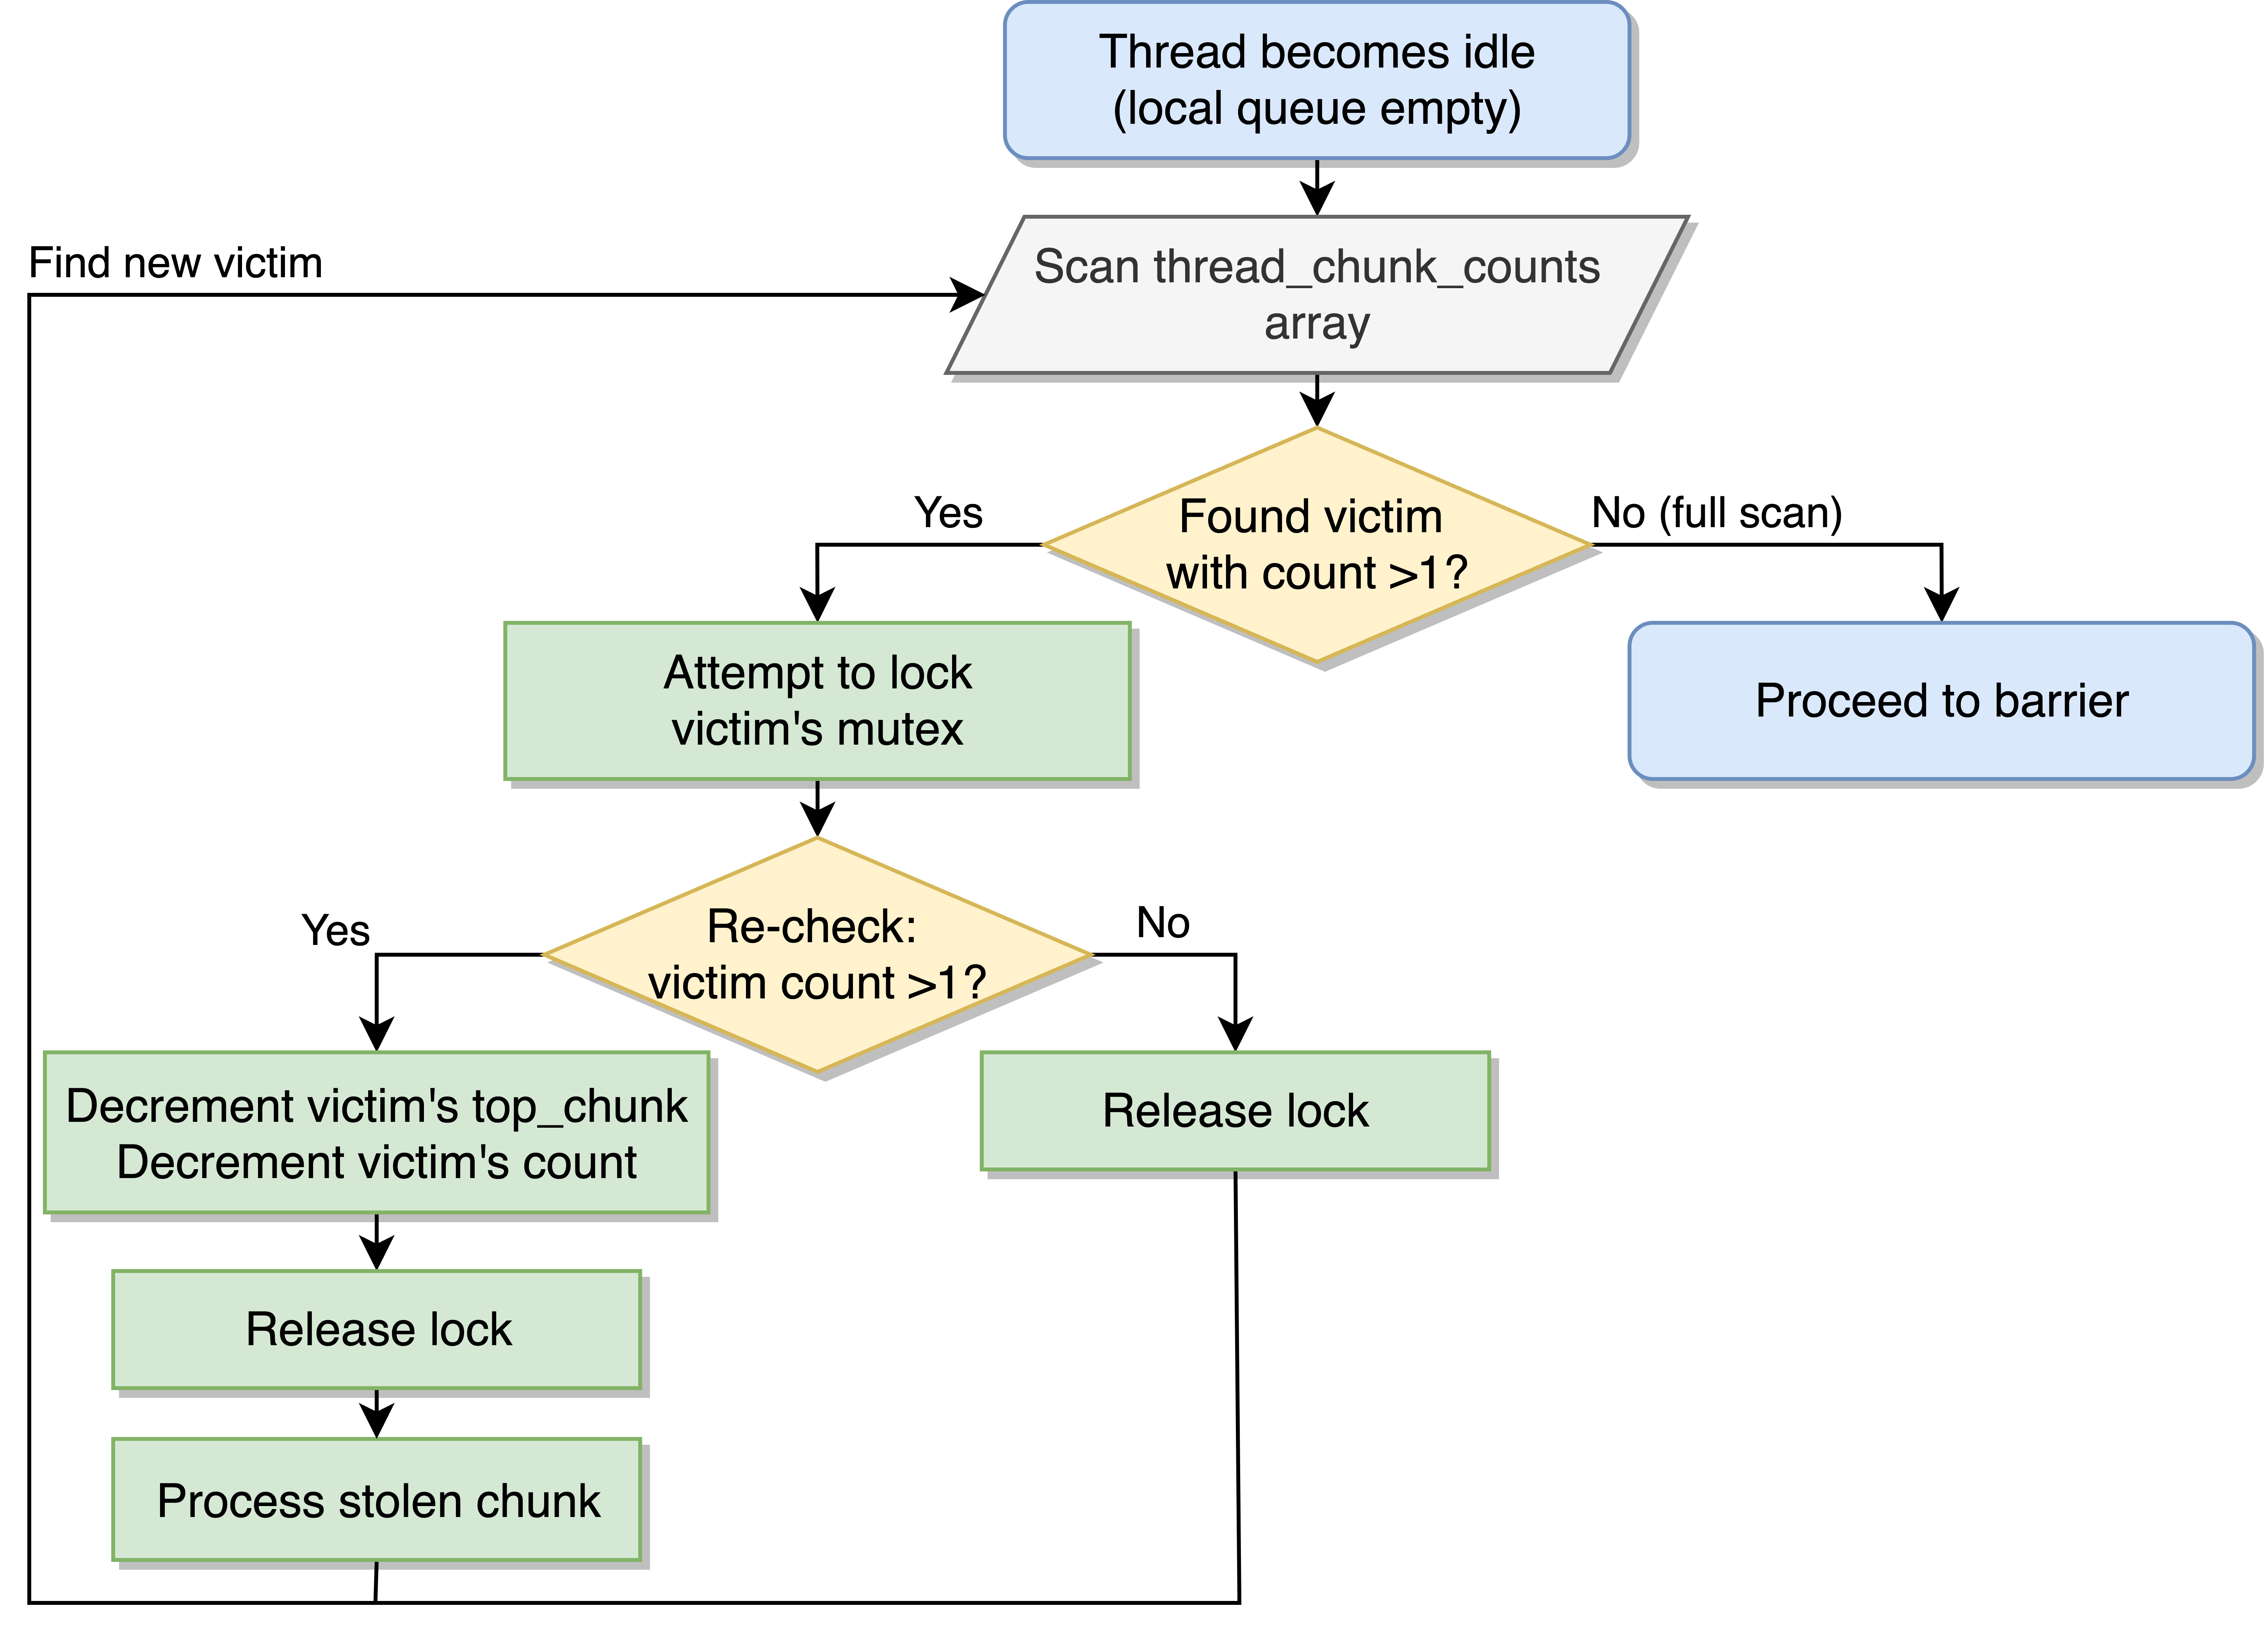
\includegraphics[width=0.7\linewidth]{images/workstealing.png}
    \caption{The work-stealing protocol.}
    \label{fig:workstealing}
\end{figure}

\subsection{Thread Pool and Work Dispatch}

The explicit parallelization of the BFS algorithm is built upon a persistent thread pool. This design is motivated by the high performance cost associated with the creation and destruction of operating system threads. By creating a fixed-size pool of worker threads once at program initialization and reusing them for each subsequent BFS traversal, the significant overhead of thread management is amortized all BFS runs. The \texttt{thread\_pool\_t} structure serves as the central control block for the entire pool, managing thread handles, state, and the synchronization primitives required for coordination between the main (parent) thread and the worker (child) threads.

\begin{minted}{c}
typedef struct {
  pthread_cond_t cond_children;    // Used to signal child threads
  pthread_mutex_t mutex_children;
  pthread_cond_t cond_parent;      // Used to signal the parent thread
  pthread_mutex_t mutex_parent;
  
  pthread_t threads[MAX_THREADS];  // Set of spawned threads
  int thread_ids[MAX_THREADS];     // Set of spawned threads' IDs
  atomic_uint run_id;              // Counter for work cycles
  atomic_bool stop_threads;        // Flag to signal threads to terminate
  atomic_bool children_done;       // Flag to signal parent that workers are done
  
  void *(*routine)(void *);        // Stores the worker function pointer
} thread_pool_t;
\end{minted}

\paragraph{Synchronization Primitives} The implementation employs two distinct pairs of mutexes and condition variables to manage the two-way communication between the main thread and the worker threads. The \texttt{cond\_children} condition variable and its associated \texttt{mutex\_children} are used exclusively to manage the state of the worker threads. The main thread signals \texttt{cond\_children} to wake the workers and dispatch a new work cycle. Symmetrically, the \texttt{cond\_parent} condition variable and \texttt{mutex\_parent} are used by the main thread. This allows it to enter an efficient wait state, blocking on \texttt{cond\_parent} until a worker signals that the entire BFS task is complete. This separation makes the synchronization logic simple, preventing potential deadlocks or race conditions that could arise from using a single set of primitives for bidirectional communication.

\paragraph{State and Signaling Variables} The coordination between threads is orchestrated through a set of atomic state variables that ensure thread-safe communication without requiring locks for every state change. The primary signaling mechanism is the atomic \texttt{run\_id} integer, which functions as a work cycle counter. Using a counter instead of a simple boolean flag provides a more robust design, as each work dispatch is identified by a unique ID. This prevents workers from accidentally performing a work cycle multiple times in the case of a spurious wakeup, as they explicitly check their local counter against the global one. The \texttt{stop\_threads} atomic boolean variable is used to signal a graceful shutdown of the pool. Finally, the \texttt{children\_done} atomic boolean variable is used to signal that the children have terminated the BFS.

\paragraph{Thread pinning} Upon creation, each thread is pinned to a specific CPU core using the Linux-specific \texttt{pthread\_setaffinity\_np} function. This overrides the default behavior of the operating system's scheduler, which may otherwise migrate threads between cores to balance the overall system load. The primary benefit of this is the enhancement of data locality. As a thread executes, it populates its core's private L1 and L2 caches with frequently accessed data, such as its stack and the graph data from its assigned work chunks. If the thread were to be migrated, these warm caches would be lost, and it would have to repopulate the cold caches of the new core, incurring significant latency from fetching data from the L3 cache or main memory \cite{gandham2024occ}.

\vspace{0.5em}
\subsubsection{Synchronization Lifecycle} \label{sec:synchronization}
The interaction between the main thread and the worker threads follows a specific order which ensures minimal busy-waiting and efficient CPU usage through the use of condition variables. The state diagram of the main and worker threads is shown in \cref{fig:synchronization}.

\paragraph{Initialization and Creation} The pool is first initialized with \texttt{init\_thread\_pool()}, which sets up the mutexes and condition variables. Subsequently, \texttt{thread\_pool\_create()} spawns \texttt{MAX\_THREADS} worker threads. Each thread is assigned a unique ID and it immediately enters a wait state. In this state, each worker thread acquires the children's mutex and enters a while loop that blocks on the \texttt{cond\_children} condition variable. A worker is only released from this wait when the global \texttt{run\_id} (controlled by the main thread) is equal to or greater than the worker's own local \texttt{run\_id}. Upon waking, the worker increments its local \texttt{run\_id}, effectively "consuming" the work signal, which prepares it to wait for the next cycle after its current task is complete.

\paragraph{Work Dispatch} The main thread initiates a BFS traversal by calling \texttt{thread\_pool\_start\_wait()}. This function acts as the dispatcher. It first acquires the necessary locks, then increments the global \texttt{run\_id}, and finally calls \texttt{pthread\_cond\_broadcast()}. This broadcast wakes up all waiting worker threads simultaneously, causing them to exit their wait state and begin executing the main BFS routine.

\paragraph{Completion and Notification} After dispatching the work, the main thread immediately blocks by calling \texttt{pthread\_cond\_wait()} on the parent's condition variable, \texttt{cond\_parent}. It remains in this sleep state, consuming no CPU cycles, until the entire BFS traversal is complete. The last worker thread to finish the final step of the BFS is responsible for calling \texttt{thread\_pool\_notify\_parent()}. This function sets the \texttt{children\_done} predicate to true and signals \texttt{cond\_parent}, waking the main thread and allowing the program to proceed.

\paragraph{Termination} To shut down the pool, the main thread calls \texttt{thread\_pool\_terminate()}. This function sets the \texttt{stop\_threads} flag to true and broadcasts one final signal on the \texttt{cond\_children} condition variable to ensure any sleeping threads wake up. The awakened threads check the \texttt{stop\_threads} flag and call \texttt{pthread\_exit} to terminate gracefully. The main thread then calls \texttt{pthread\_join} on all worker threads to guarantee they have all exited before the program's resources are deallocated.

\begin{figure}
    \centering
    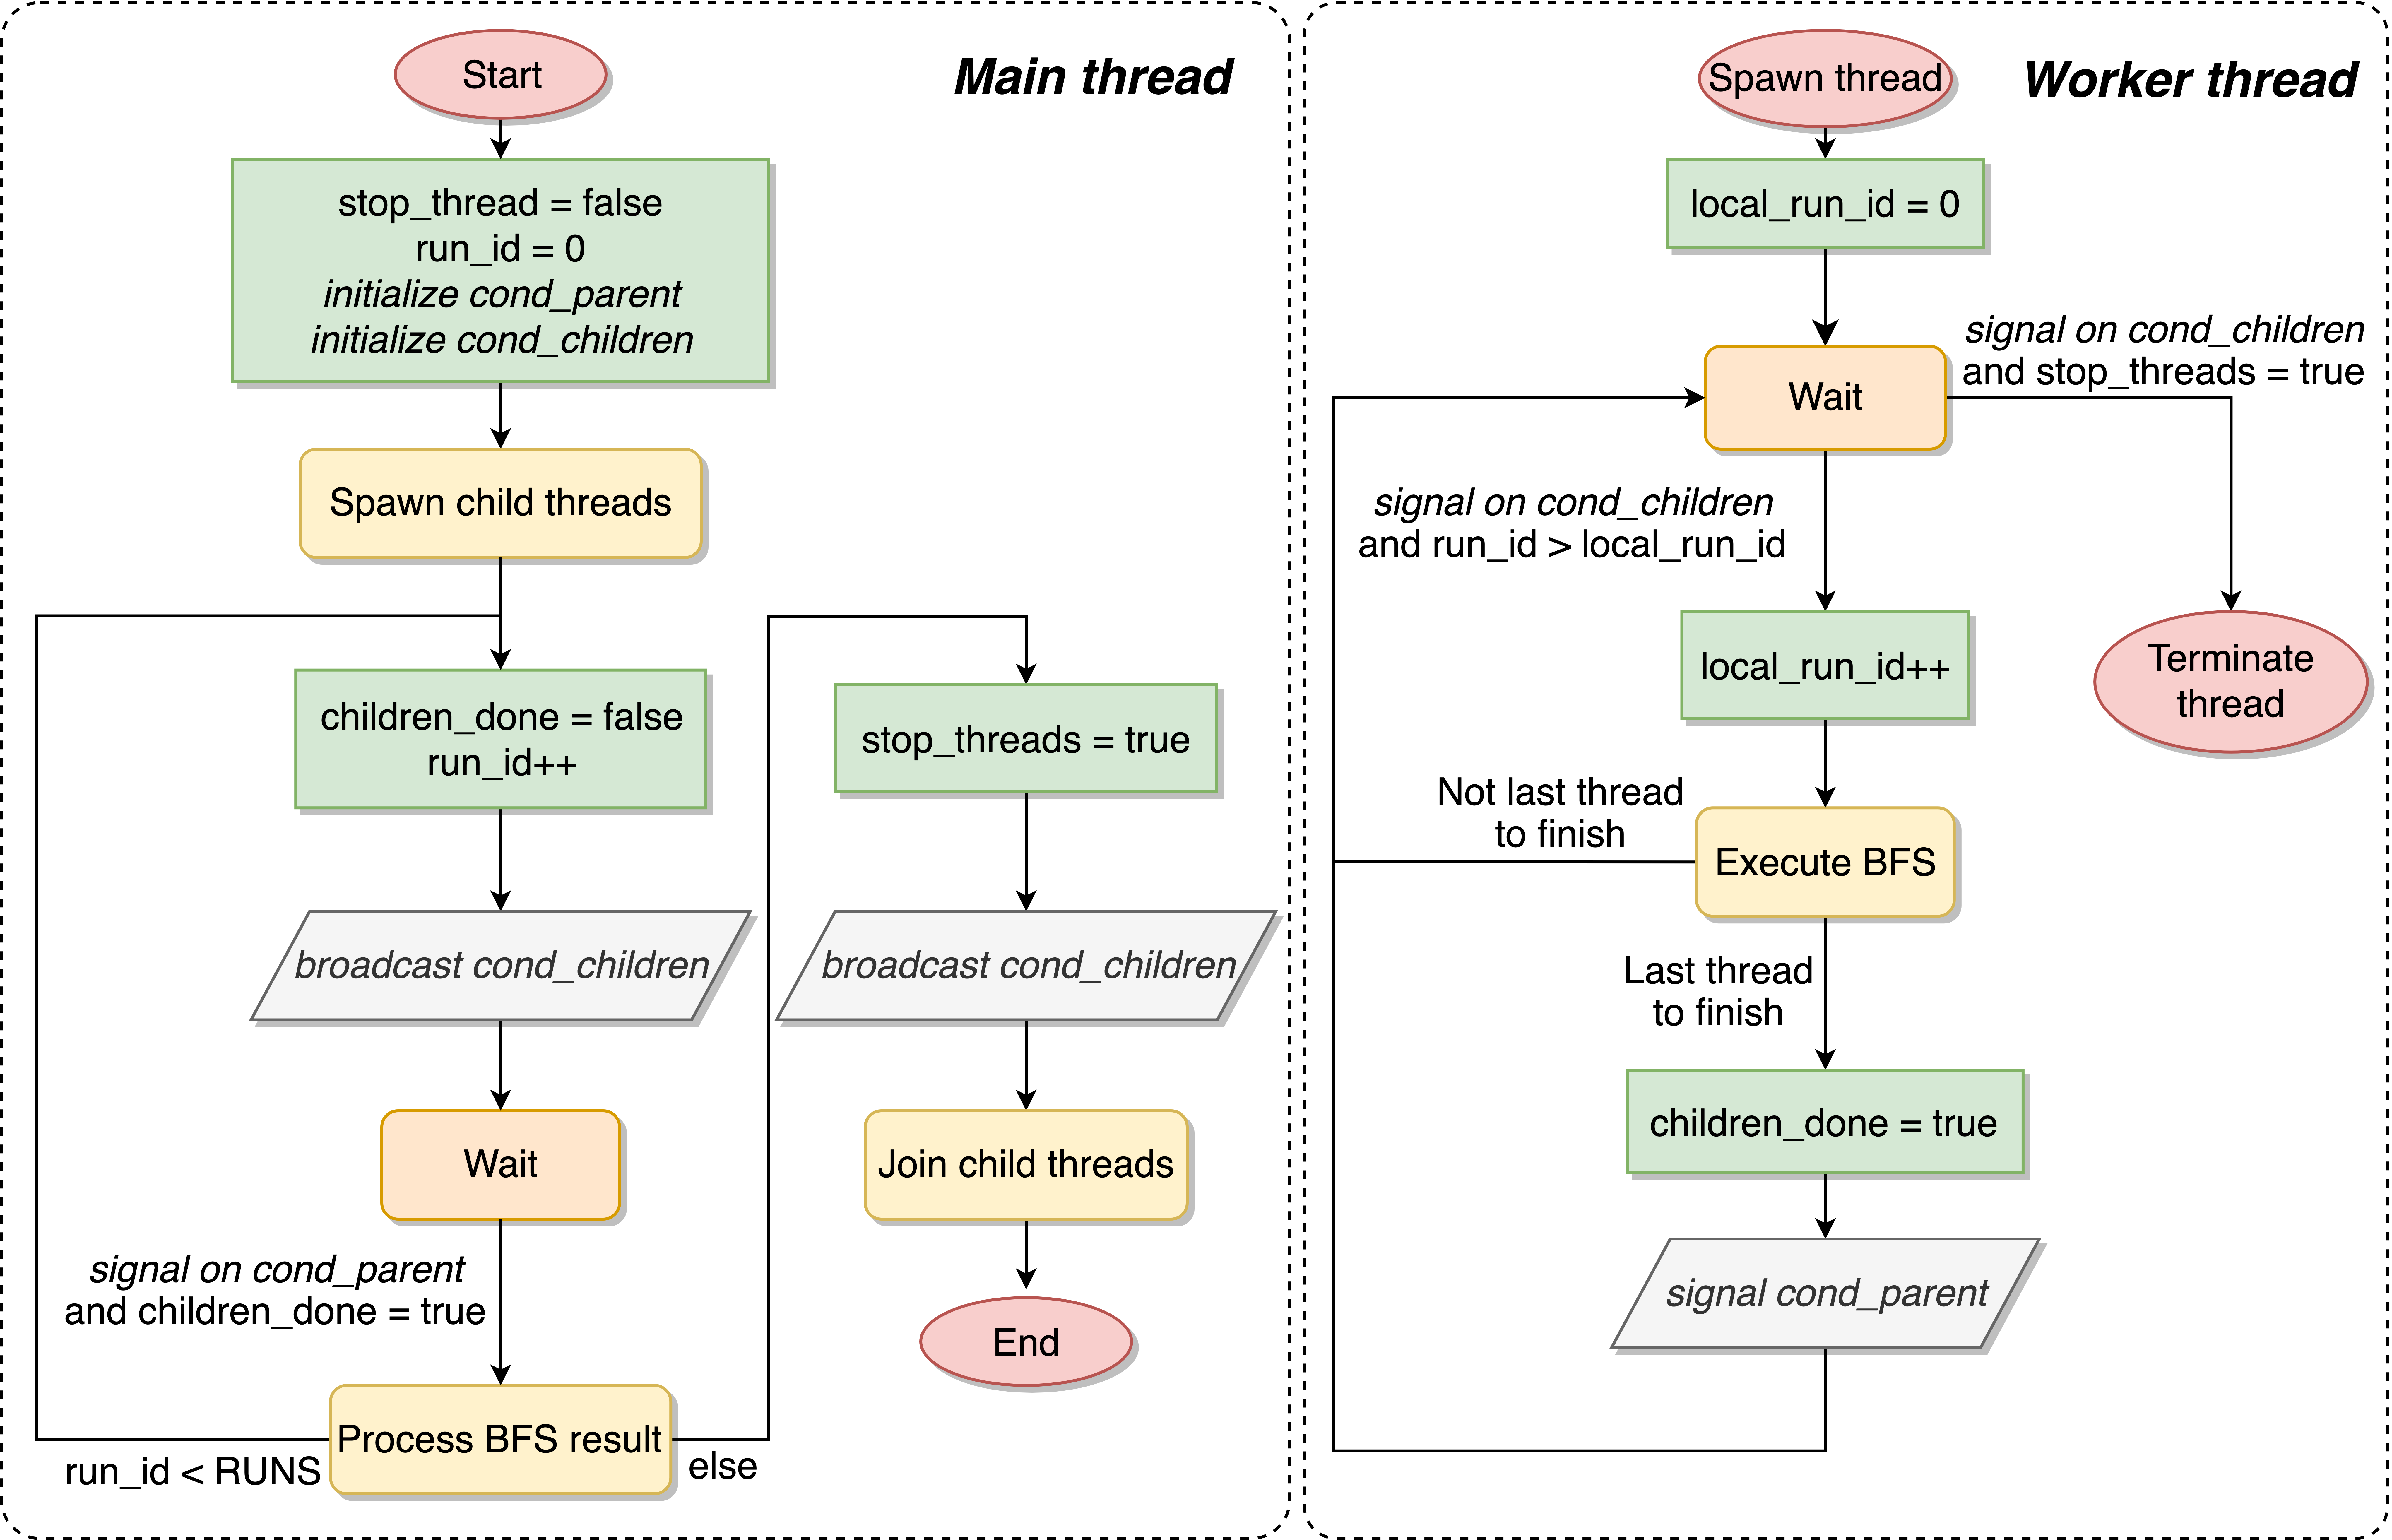
\includegraphics[width=0.9\linewidth]{images/threads.png}
    \caption{State diagrams of the main and worker threads. The \texttt{RUNS} variable contains the total number of iterations of the BFS.}
    \label{fig:synchronization}
\end{figure}

\subsection{Level Synchronization and Barrier Implementation}

The level-synchronous BFS requires a barrier, which ensures all threads have completed their work for the current level before any thread begins processing the next. This implementation uses a custom barrier that is a variation of the Sense-Reversal Centralized Barrier.

The synchronization is managed using an atomic counter, \texttt{active\_threads}, and the \texttt{distance} variable. At the beginning of each level, \texttt{active\_threads} is reset to \texttt{MAX\_THREADS}. When a thread finishes processing all of its work for the current level (including any stolen work), it atomically decrements this counter.

The last thread to finish its work is designated the "leader" for that level. The thread notices that it is the leader because the \texttt{active\_threads} variable is equal to one when it arrives at the barrier. This leader thread is responsible for performing the serial tasks required between levels: swapping the pointers for the current and next frontiers, checking if the new frontier is empty to determine if the entire BFS should terminate, and finally, incrementing the global \texttt{distance} variable. If there are no vertices left in the frontier, instead of incrementing the global \texttt{distance} variable, it sets the \texttt{exploration\_done} boolean variable and notifies the main thread that the BFS has terminated (as explained in \cref{sec:synchronization}).

The other, non-leader threads, after decrementing the counter, enter a spin-wait loop, continuously checking if the distance has been incremented by the leader. The act of incrementing distance serves as the "sense-reversal" signal, releasing all waiting threads from the barrier simultaneously to begin work on the next level. This design avoids the overhead associated with \texttt{pthread\_barrier\_t} objects as it relies on a single atomic counter and a shared variable for coordination.

\begin{figure}[H]
    \centering
    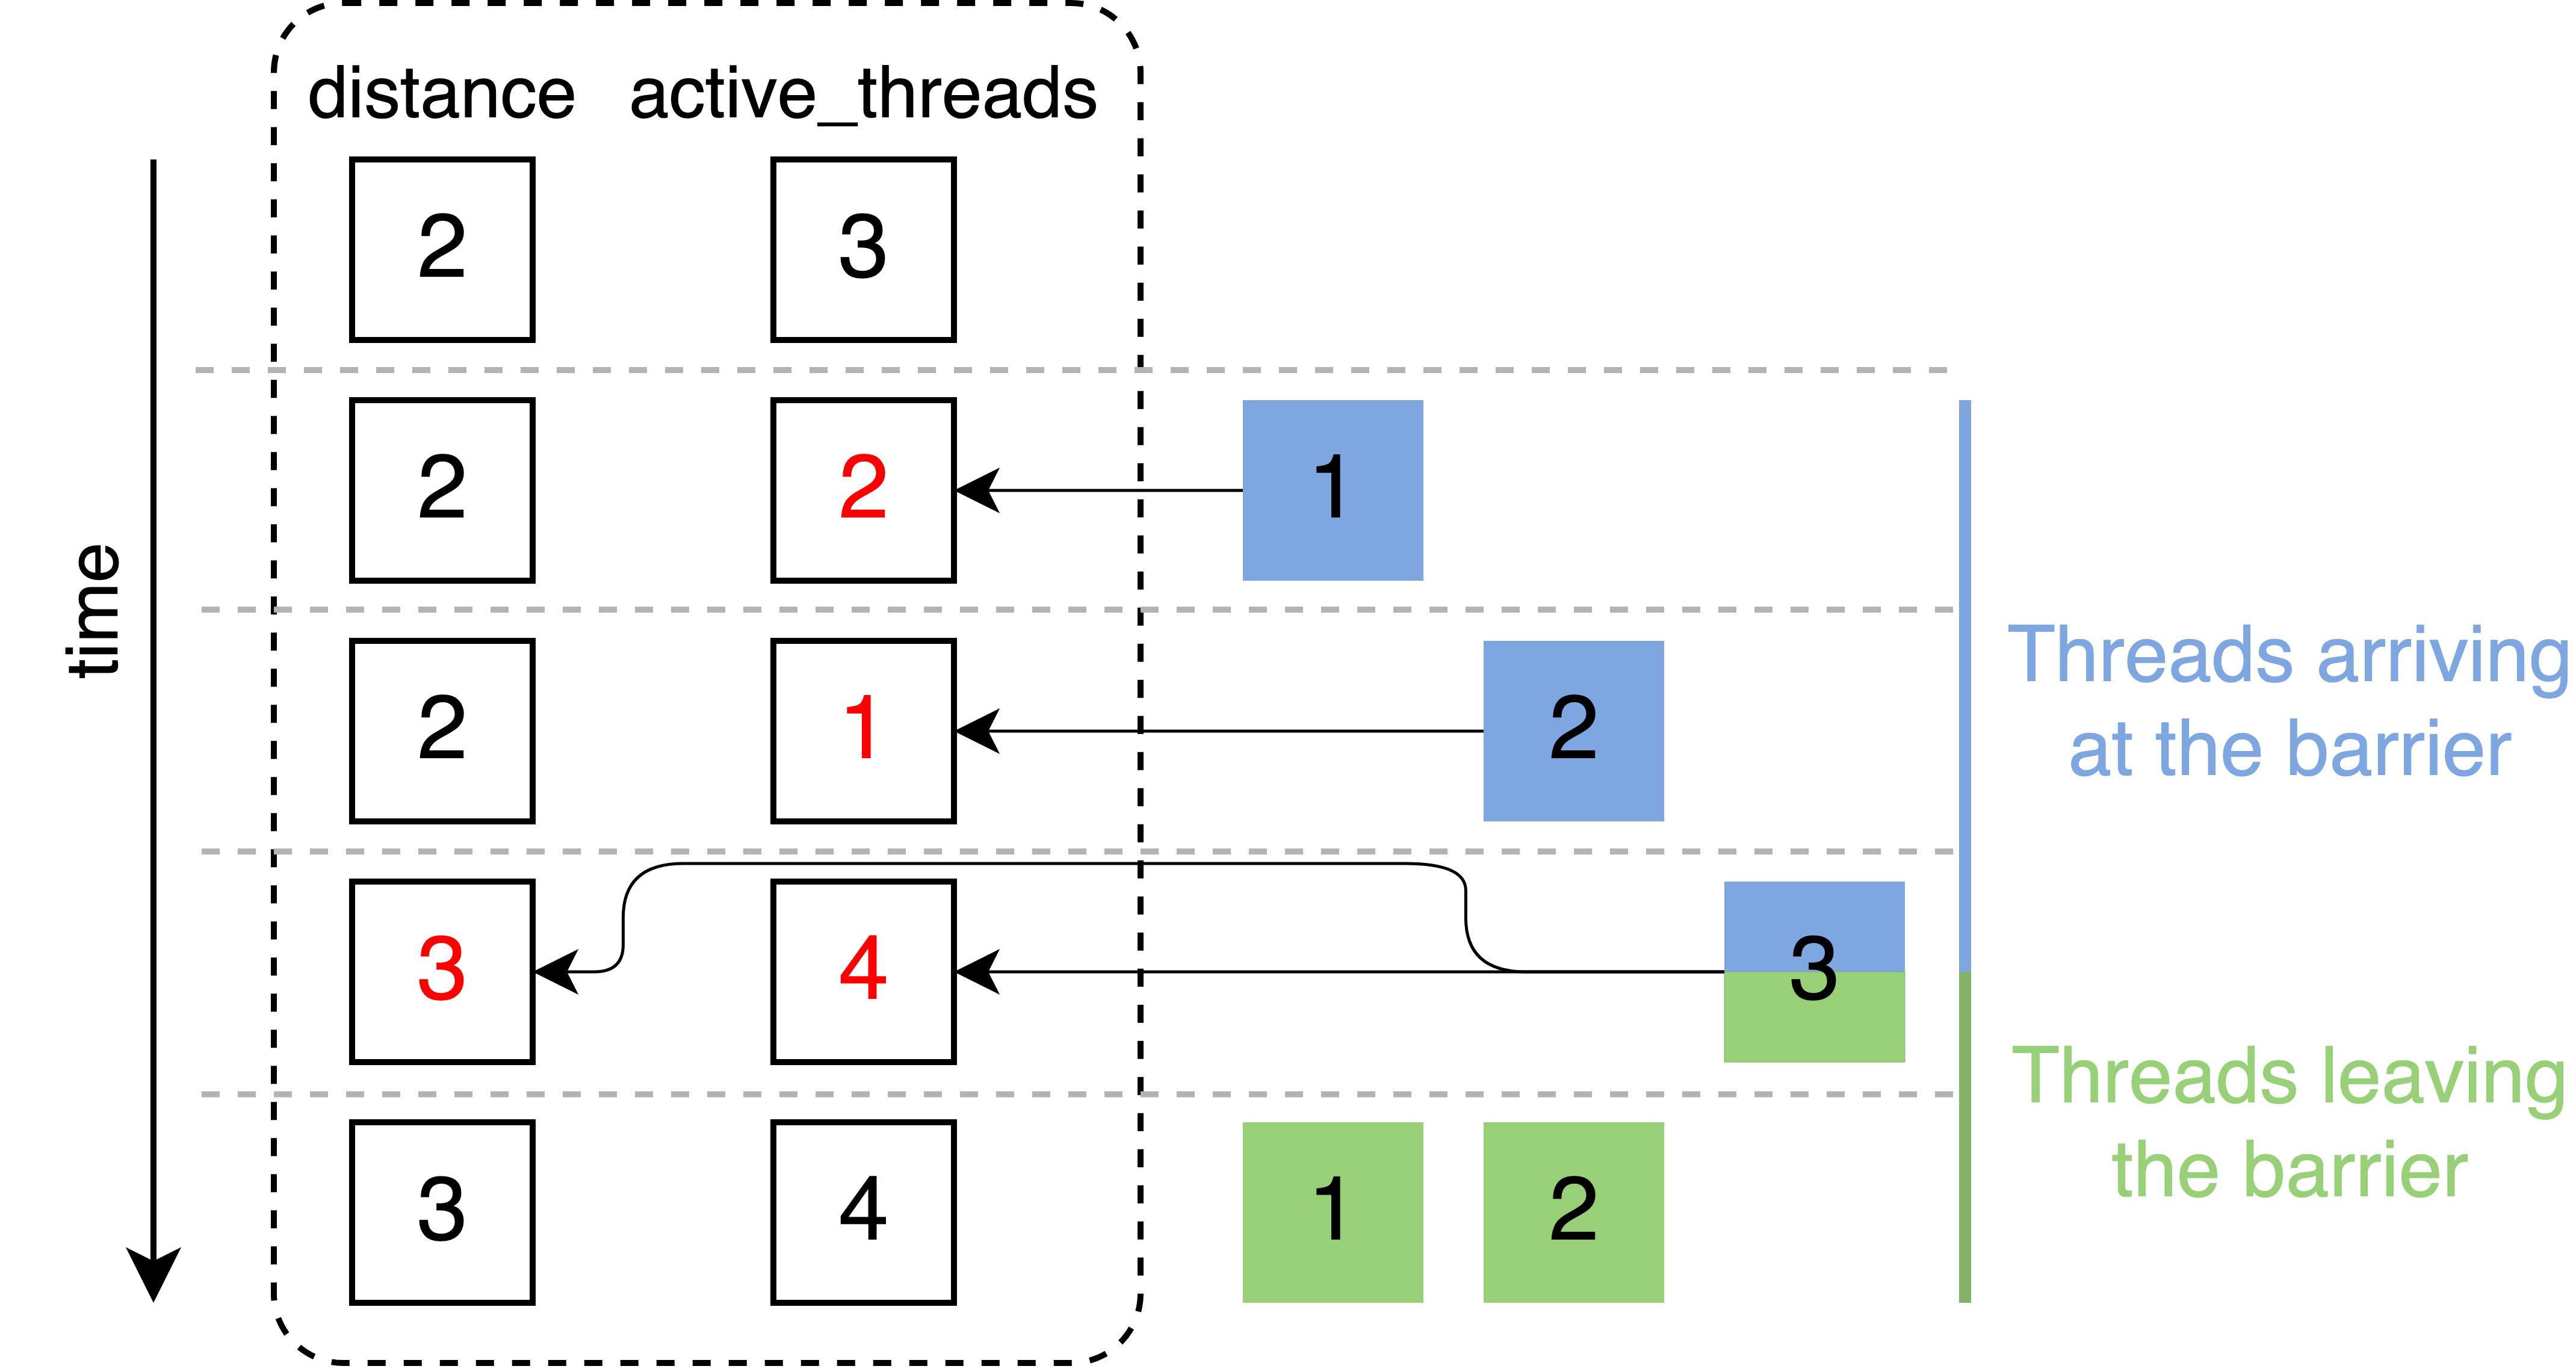
\includegraphics[width=0.6\linewidth]{images/barrier.png}
    \caption{The barrier during a BFS exploration at \texttt{distance = 2} with 3 worker threads. When threads arrive at the barrier (shown in blue), they decrement the \texttt{active\_threads} variable (changes to variables are marked in red) and spin-wait until the \texttt{distance} variable changes. When the last thread arrives at the barrier, it increments the \texttt{distance} and resets \texttt{active\_threads}, thus releasing all the waiting threads (shown in green).}
    \label{fig:barrier}
\end{figure}
\null
\vfill
